\section{Proof}

\begin{frame}{Proof.}
	TODO proof.
\end{frame}

\begin{frame}{Proof of $\impliedby$ (Off The Dome.)}
	Let $G' = (V',E')$ be the signed graph for $\sigma_m'$. We insert a new vertex $v$ into $G'$, and connect it to the vertices $v_2,\dots,v_{d_1+m+1}$ via a positive edge, and $v_{p-m+1},\dots,v_p$ via a negative edge. The resulting new vertex would have degree
	\begin{equation*}
		(d_1+m)-(m) = d_1
	\end{equation*}
	as required.
\end{frame}

\begin{frame}{$\impliedby$ Diagram}
	\begin{figure}[H]
        \centering
        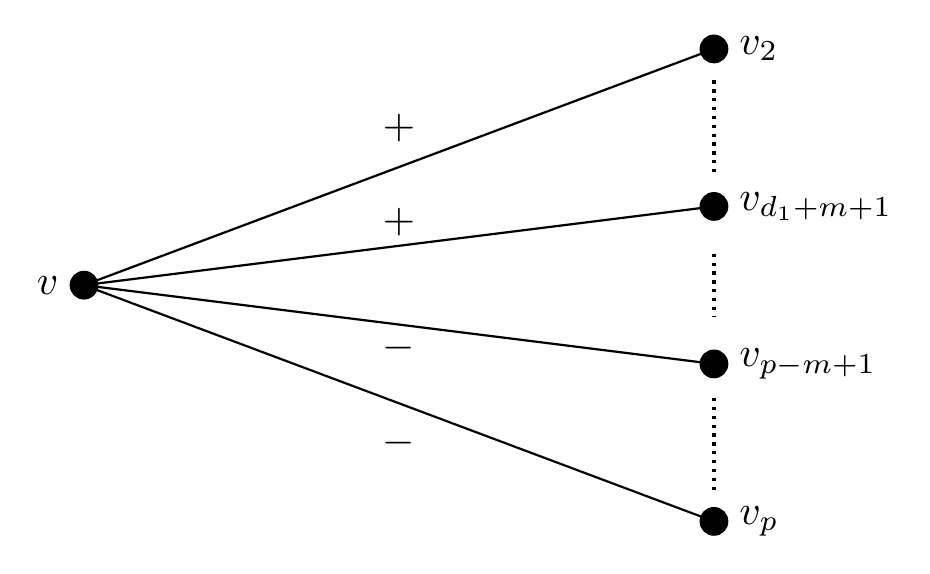
\begin{tikzpicture}[scale=1]
            %graph
			\draw[fill] (-4,0) circle (5pt);

            \node[left] at (-4.2,0) {\(\scalebox{1.5}{\(v\)}\)};

			\draw[fill] (4,3) circle (5pt);

			\node[right] at (4.2,3) {\(\scalebox{1.5}{\(v_2\)}\)};

			\draw[very thick, dotted] (4,2.6)--(4,1.4);

			\draw[fill] (4,1) circle (5pt);

			\node[right] at (4.2,1) {\(\scalebox{1.5}{\(v_{d_1+m+1}\)}\)};

			\draw[fill] (4,-3) circle (5pt);

			\node[right] at (4.2,-3) {\(\scalebox{1.5}{\(v_{p}\)}\)};

			\draw[very thick, dotted] (4,-2.6)--(4,-1.4);

			\draw[fill] (4,-1) circle (5pt);

			\node[right] at (4.2,-1) {\(\scalebox{1.5}{\(v_{p-m+1}\)}\)};

			\draw[very thick, dotted] (4,0.4) -- (4,-0.4);

			\draw[thick] (-4,0)--(4,3);

			\node[above] at (0,1.7) {\(\scalebox{1.5}{\(+\)}\)};

			\draw[thick] (-4,0)--(4,1);

			\node[above] at (0,0.5) {\(\scalebox{1.5}{\(+\)}\)};

			\draw[thick] (-4,0)--(4,-1);

			\node[below] at (0,-0.5) {\(\scalebox{1.5}{\(-\)}\)};

			\draw[thick] (-4,0)--(4,-3);

			\node[below] at (0,-1.7) {\(\scalebox{1.5}{\(-\)}\)};
        \end{tikzpicture}
    \end{figure}
\end{frame}

\begin{frame}{Setup for $\implies$}
	Suppose $\sigma$ is the signed degree sequence of a signed graph $G = (V,E)$, where $V = \{v_1,\dots,v_p\}$ and $d_i = sd(v_i)$. For each $0 \leq s \leq \frac{p-1-d_1}{2}$, define the signed degree sequence
	\begin{equation*}
		\sigma_s' : d_2-1,\dots,d_{d_1+s+1}-1,d_{d_1+s+2},\dots,d_{p-s},d_{p-s+1}+1,\dots,d_p+1
	\end{equation*}
	By the previous theorem, this sequence is graphical for at least one $s$. In particular, we choose $s$ to minimize $|s-m|$, and call the associated signed graph $G' = (V',E')$. We proceed now by contradiction.
\end{frame}

\begin{frame}{Case 1 : $s < m$}
	By construction, $d_{d_1+s+2} > d_{p-s}$ since $s+1 \leq m$ and our sequence is in standard form. Set $a = d_1+s+2, b = p - s$. We end up with one of the following subcases.
	\begin{enumerate}
		\item $\exists x \in V'\backslash\{v_a,v_b\}$ such that $v_ax^{+}, v_bx^{-} \in E'$. Then remove both these edges from $G'$ to get the signed degree sequence $\sigma_{s+1}'$, making $\sigma_{s+1}'$ graphical and contradicting the minimality of $|s - m|$.
		\item $\exists x \in V'\backslash\{v_a,v_b\}$ such that $v_ax^{+} \in E'$, $v_bx^{\pm} \notin E'$. Then remove $v_ax^{+}$ and add $v_bx^{+}$ to get the signed degree sequence $\sigma_{s+1}'$.
		\item $\exists x \in V'\backslash\{v_a,v_b\}$ such that $v_bx^{-} \in E'$, $v_ax^{\pm} \notin E'$. Then remove $v_bx^{-}$ and add $v_ax^{-}$ to get the signed degree sequence $\sigma_{s+1}'$.
	\end{enumerate}
\end{frame}


\begin{frame}
	Under each of these subcases, here's how the signed degree sequences change under adding/removing the mentioned edges. Notice that in each case, $sd(x)$ stays constant.
	\begin{align*}
		\sigma^\prime_s&: d_2-1, \dots, d_{d_1+s+1}-1, d_{a}, \dots, d_{b}, d_{p-s+1}+1, \dots, d_p+1 \\
			& \leadsto d_2-1, \dots, d_{d_1+s+1}-1, \color{red} d_{a} - 1 \color{black}, \dots, \color{red} d_{b} + 1 \color{black}, d_{p-s+1}+1, \dots, d_p+1
	\end{align*}
\end{frame}


\begin{frame}{Case 2 : $s > m$}
	By construction, $d_{d_1+s+1} \leq d_{p-s+1}$, so since $s > m$ and our sequence is in standard form we get by the maximality of $m$ that $d_{d_1+s+1} = d_{p-s+1}$, so $d_{d_1+s+1}-1 < d_{p-s+1}+1$. Set $a = d_1+s+1, b = p-s+1$. We end up with one of the following subcases.
	\begin{enumerate}
		\item $\exists x \in V'\backslash\{v_a,v_b\}$ such that $v_ax^{-}, v_bx^{+} \in E'$. Then remove both these edges from $G'$ to get the signed degree sequence $\sigma_{s-1}'$, making $\sigma_{s-1}'$ graphical and contradicting the minimality of $|s - m|$.
		\item $\exists x \in V'\backslash\{v_a,v_b\}$ such that $v_ax^{-} \in E'$, $v_bx^{\pm} \notin E'$. Then remove $v_ax^{-}$ and add $v_bx^{-}$ to get the signed degree sequence $\sigma_{s-1}'$.
		\item $\exists x \in V'\backslash\{v_a,v_b\}$ such that $v_bx^{+} \in E'$, $v_ax^{\pm} \notin E'$. Then remove $v_bx^{+}$ and add $v_ax^{+}$ to get the signed degree sequence $\sigma_{s-1}'$.
	\end{enumerate}  \qed
\end{frame}
